% !TeX program = lualatex
\chapter{Theoretischer Hintergrund} % Main chapter title
\label{Background} % For referencing the chapter elsewhere, use \ref{Background}
Um in den folgenden Kapiteln ein grundlegendes Verständnis der Begrifflichkeiten, Zusammenhänge und Konzepte gewährleisten zu können, ist es notwendig,
diese vorab zu definieren und einzugrenzen. Da sich diese Arbeit mit der Privatsphäre von Stakeholdern in einem Softwareentwicklungsunternehmen beschäftigt,
ist es zunächst erforderlich, die Grenzen der Privatsphäre klar zu definieren und anhand dieser, eine Messung zu schaffen. Da diese Messung durch die persönlichen Daten
der einzelnen Stakeholder erfolgt, werden Daten im Allgemeinen ebenfalls auf dieses Feld begrenzt und der Umgang mit diesen erklärt. Was Stakeholder sind und welche in dieser Analyse
relevant sind, ist ebenfalls ein erforderlicher Schritt zum grundlegenden Verständnis dieser Arbeit. Im Anschluss werden DevOps definiert und mithilfe gewählter Beispiele in der Praxis erläutert.

\section{Die Privatsphäre - eine Eingrenzung}
Der Begriff Privatsphäre ist im Wortschatz der deutschen Sprache tief verankert und findet im Alltag in vielerlei Hinsicht Gebrauch: Menschen decken Notebook- und Smartphonekameras
ab, protestieren gegen Überwachungskameras im öffentlichen Raum \cite{Stallwood:2013aa} oder möchten nicht, dass ihre persönlichen und privaten Daten auf sozialen Netzwerken ohne ihre Zustimmung
bzw. ohne ihre Kenntnis verbreitet werden \cite{Picchi:2018aa} - eine grundlegende, allgemeine Kenntnis der Privatsphäre ist also präsent, aber wie lässt sich diese definieren? \newline
Die Privatsphäre lässt sich erklären als einen eingegrenzten, nicht-öffentlichen Raum, in welchem ein Individuum bzw. Individuen nach eigenem Belieben, ohne äußere Einflüsse oder der Beobachtung durch
Unbeteiligte, zur freien Entfaltung der eigenen Person, handeln kann bzw. können \cite*{Pettinger:2020aa}. Möchte man diese Definition nun auf die Softwareentwicklung übertragen, so müssen die möglichen, 
vorherrschenden Komponenten von persönlichen Daten näher betrachtet werden: In Unternehmen, welche sich mit der Softwareentwicklung befassen, müssen Daten vorhanden sein, welche Individuen einzigartig 
bestimmen können - dies kann in Form von IDs und individuell gewählten Nutzernamen vorzufinden sein, aber auf der Kehrseite auch mit Klarnamen, E-Mail Adressen sowie eindeutig identifizierbaren IDs. Schließlich 
möchte man einzelne, erledigte Arbeiten innerhalb der Angestellten unterscheiden können. \newline
Nichtsdestotrotz wird es dadurch nicht leichter, Privatsphäre im Allgemeinen greifbar zu machen - diese ist nämlich \enquote{vollständig determiniert durch die Bereitschaft zur persönlichen Offenlegung von bestimmten Menschen in einer
bestimmten Gemeinschaft und zu einer bestimmten Zeit} \cite{Miller:2000aa}. In einer vereinfachten Ausdrucksweise bedeutet dies, dass jedes Individuum oder jede Gemeinschaft, eigene, selbst deklarierte Grenzen zum Veröffentlichen
der eigenen persönlichen Daten besitzt und diese untereinander auch variieren können. \newline
Auf diese Definition und Eingrenzung der Privatsphäre wird in den folgenden Kapiteln dieser Analyse Bezug genommen.

\section{Persönliche Daten am Arbeitsplatz} \label{personaldata}
In Hinblick auf aktuelle Arbeitsumgebungen in Softwareentwicklungsunternehmen ist bereits seit mehreren Jahren bekannt, dass eine Auswertung der persönlichen Daten (beispielsweise in DevOps-Tools) in den alltäglichen Arbeitsablauf herangewachsen ist. Grund hierfür ist schlichtweg die Natur dieser Arbeit in einem Softwareentwicklungsunternehmen: \newline
Vorgesetzte haben schließlich das Recht sicherzustellen, dass ihre Angestellten ihrer Arbeit bis zu einem bestimmten Grad zufriedenstellend nachgehen \cite{Miller:2000aa} - aber auch in Bezug auf die Allgemeinheit am Arbeitsplatz ist dieser Aspekt nicht irrelevant, da Angestellte nicht härter arbeiten möchten als erforderlich, um die Arbeit von inkompetenten
Kollegen ausgleichen zu müssen \cite{Miller:2000aa}. Die Arbeit in einem Softwareentwicklungsunternehmen kann schließlich nur erschwert nachvollzogen werden, da die bloße Anwesenheit am Arbeitsplatz hierfür meistens nicht ausreicht. Der Angestellte könnte beispielsweise an seinem Arbeitsrechner sitzen, aber seine gesamte Arbeitszeit durch arbeitsirrelevante
Unterhaltungen mit Kollegen im internen Kommunikationstool verbringen. \newline Trotzdem muss das Recht auf Privatsphäre jedes Individuums berücksichtigt bzw. respektiert werden und kann nicht durch die bloße autoritäre Natur eines Vorgesetzter-Angestellten-Verhältnisses relativiert werden. \newline 
Diese Gründe verdeutlichen das Dilemma, welches sich in Bezug auf die Privatsphäre, und damit verbunden die persönlichen Daten, am Arbeitsplatz herauskristallisiert: Wie weit kann bzw. muss das Unternehmen (also die Führungsebene, aber auch die Kollegen), um einen grundlegenden und annehmbaren Arbeitsfluss zu gewährleisten, und wie weit können bzw. müssen die
einzelnen Individuen, welche zu diesem Unternehmen beitragen, von ihren eigenen persönlichen Daten für dieses Vorhaben preisgeben? \newline
Aktuelle Arbeiten zu dem Aspekt der Privatsphäre und der Überwachung persönlicher Daten sind zu dem Entschluss gekommen, dass \enquote{Mitarbeiter [insbesondere aus dem DevOps-Bereich] einem besonderen Risiko der datengetriebenen Überwachung ausgesetzt [sind]} \cite{Federrath:2020aa}, da schlichtweg die Unterstützung von diversen Tools zu diesem Thema heutzutage
existiert und eine empirisch nachgewiesene Bereitschaft zur Erfassung und Auswertung von (persönlichen) Daten gewährleistet ist \cite{Federrath:2020aa}: Durch einer von Bitkom Research durchgeführten Studie wurde 2015 erwiesen, dass beispielsweise in den Personalabteilungen von jedem zweiten Unternehmen (hier: in der Softwareentwicklung) Bewerber (ohne eigene Kenntnisnahme)
über soziale Netzwerke überprüft werden oder \enquote{Big Data}-Analysen zunehmend für Kernaufgaben zum Einsatz kommen \cite{Research:2015aa}.

\section{Stakeholder}
\begin{marginfigure}[1\baselineskip]
    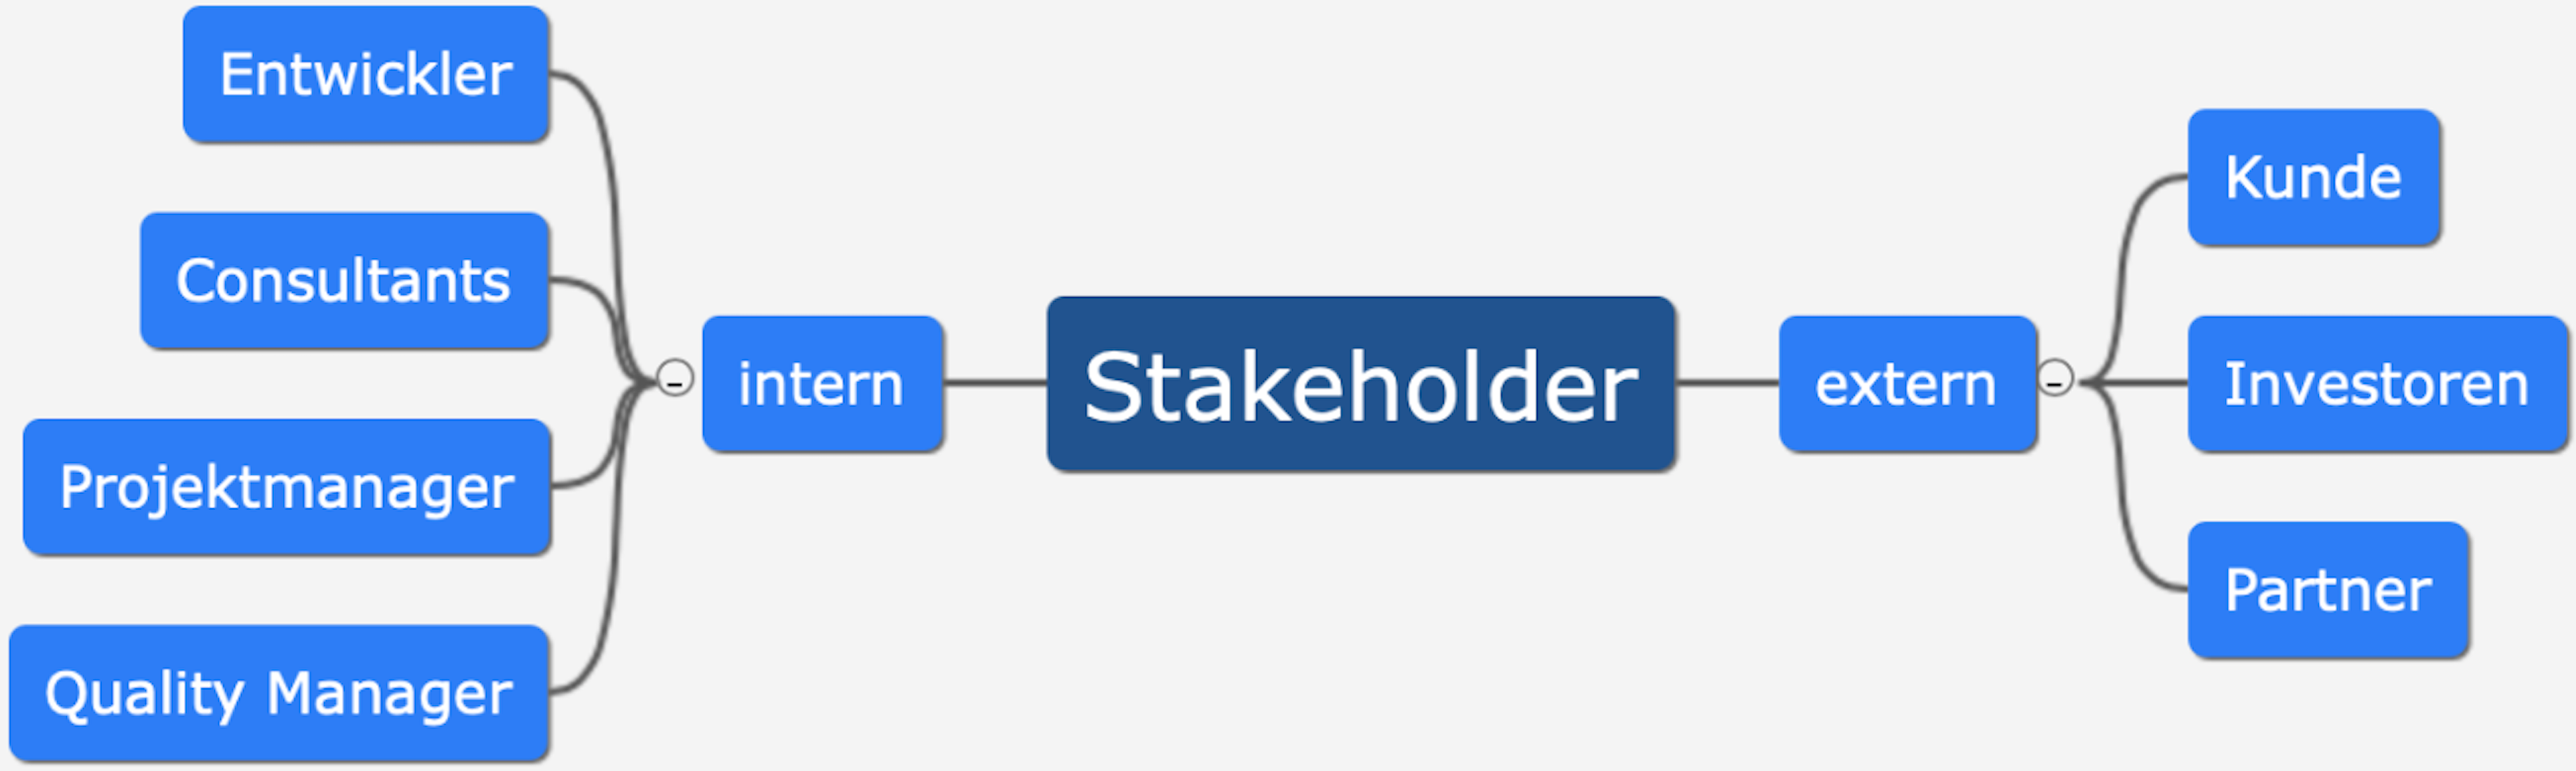
\includegraphics[width=1.4\marginparwidth]{stakeholder.png}
    \caption{Beispielhafte Stakeholder-Mindmap.}
\end{marginfigure}
Der Begriff \enquote{Stakeholder} lässt sich neben der Informatik auch in der Betriebswirtschaftslehre vorfinden - das Bindeglied der beiden Bereiche in diesem Aspekt repräsentieren Unternehmen im Allgemeinen.
Da diverse Institutionen, Personen und Personengruppen Erwartungen an Unternehmen haben und eigene Interessen vertreten, stellen Stakeholder jene \enquote{[...] [dar], die von den Aktivitäten eines Unternehmens 
direkt oder indirekt betroffen sind oder [...] ein Interesse an diesen [...] haben} \cite{Fleig:2016aa}. Als Beispiele können diese in Form von Kunden und Lieferanten bis zu eigenen Mitarbeitern und Eigentümern (von 
Unternehmensanteilen oder vom Unternehmen selbst) auftreten \cite{Fleig:2016aa}. \newline Neben den Stakeholdern selbst existiert der sogenannte \enquote{Stakeholder-Ansatz}: Dieser besagt die Betrachtung einer Unternehmung
als Organisation unter Zusammenschluss verschiedener Stakeholder \cite{Seyfriedt:2018aa}. Dabei stellt die Unternehmensleitung die Vermittlung zwischen den verschiedenen Gruppen dar \cite{Seyfriedt:2018aa}. \newline
Betrachtet man diesen Begriff nun aus der informatischen Sicht, so kann man aus der Definition herleiten, dass Stakeholder hier in der Regel Erwartungen und Interessen an einem einem Programm bzw. einer Applikation oder einem 
Computersystem, statt einem Unternehmen verfolgen. \newline In dieser Analyse ist der Bezug fortlaufend auf diese Stakeholder gelegt, da diese die befragten Experten darstellen.

\section{DevOps}
\enquote{Die Zufriedenheit unserer Kunden liegt uns am Herzen} - durch dieses Motto strahlen Unternehmen ihre Kundenorientierung aus und möchten in der Regel zusätzlich durch Feedback, Kulanz, einem überzeugenden Produkt
oder einem allgemein positiv zurückgebliebenem Eindruck beim Kunden überzeugen. In Softwareentwicklungsunternehmen vereint DevOps die benötigten Technologien, die Prozesse und die Menschen miteinander, um für diese Kunden 
andauernd hochwertige Produkte anbieten zu können \cite{MSAzure:2020aa}. \newline Der Begriff setzt sich zusammen aus \enquote{Development} (dt. \textit{Entwicklung}) von Software sowie \enquote{Operations} (dt. \textit{Vorgänge}), welche damit zusammenhängen 
\cite{MSAzure:2020aa} und repräsentiert dabei die \enquote{Zusammenarbeit von Entwicklung und Betrieb} \cite{Hasselbring:2015aa}. Dies erfolgt durch die Einführung von DevOps-Methoden und -Tools (welche nachfolgend erläutert werden), sodass den zuvor getrennten Bereichen (z.B. der Qualitätssicherung, Sicherheit etc.) die Möglichkeit zur Koordination und Zusammenarbeit geboten wird \cite{MSAzure:2020aa}. \newline Im Folgenden werden beispielhaft repräsentative DevOps-Methoden und -Tools definiert und aufgelistet.

\subsection{Continuous Integration}
In der Softwareprogrammierung ist es mit zunehmender Komplexität und Umfang des Programms üblich, mehrere einzelne Module in dieses einzubinden, weswegen sich die gängige Vorgehensweise in der Softwareentwicklung insofern gestaltet, dass das Gesamtprojekt,
welches aus diesen einzelnen Modulen besteht, durch mehrere Teams parallel vorangetrieben wird \cite{HJL:2018aa}. \newline Statt auf eine täglich erfolgende Kompilierung auf einem extra angelegten \enquote{Build}-Server warten zu müssen, kommen heutzutage in modernen
Unternehmen die sogenannte \enquote{Continuous Integration} (dt. \textit{Kontinuierliche Integration}, kurz: CI) zum Einsatz \cite{HJL:2018aa}: Diese bezeichnet \enquote{eine Technik der agilen Softwareentwicklung [...], [welche die] in kleinen Schritten vorgenommenen Änderungen [...] 
regelmäßig zusammenführt} \cite{Dirk:2018aa}, also eine kontinuierliche Integration von Softwarekomponenten wie z.B. eines Guided User Interfaces (dt. \textit{grafische Benutzeroberfläche}, kurz: GUI), eines Application Programming Interfaces (dt. \textit{Programmierschnittstelle}) etc.,
in das gemeinsame Projekt bzw. den gemeinsamen Code \cite{HJL:2018aa}. \newline Dies erfolgt in der Regel unter Einsatz von einem sogenannten \enquote{Trunk}, also der \enquote{Stamm}, welches das Hauptverzeichnis der Entwicklung des Projekts darstellt  und \enquote{Branches}, die als 
\enquote{Äste} bzw. Verzweigungen angesehen werden können und die untergeordneten Verzeichnisse der Hauptentwicklung repräsentieren \cite{Peters:2015aa}. \newline In der Arbeit im Team kann der Code dann für dasselbe Projekt also nicht erst wie zuvor nach dem Fertigstellen der anderen 
Teilbereiche mit in den Gesamtcode des Projekts aufgenommen werden, sondern nach eigenem Bedarf, sogar mehrmals am Tag \cite{Dirk:2018aa}. Dadurch kann der Code für die beteiligten Programmierer schon viel früher offengelegt werden, sodass Tests und damit verbunde Fehlerbehebungen früher 
und effizienter, durch Einsparung von Zeit und Ressourcen, durchgeführt werden können. \newline Trotzdem ist zunächst eine Umorientierung erforderlich ist, da ein bereits gängiger Prozess neu aufgelegt und zusätzliche Prozesse sowie Server neu eingebunden werden müssen \cite{HJL:2018aa, Dirk:2018aa}. 
Dieser gesamte Prozess funktioniert durch das Einspeisen der zusammengefügten Änderungen des Codes in ein Repository, womit im Anschluss eine Versionskontrolle durch die Übernahme von einer aktuellen Version des Codes durch einen automatisierten Build-Prozess \cite{HJL:2018aa} erfolgt.
\begin{marginfigure}[1\baselineskip] % move figure up by 1 line
    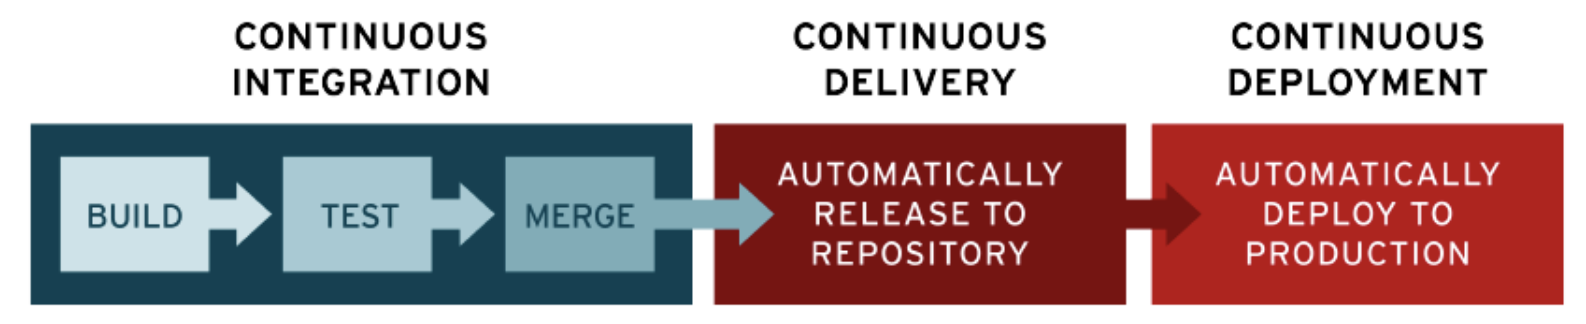
\includegraphics[width=1.4\marginparwidth]{pipeline.png}
    \caption{\label{fig:pipeline}Die CI-/CD-Pipeline \cite{RedHat:2020aa}.}
\end{marginfigure}

\subsection{Continuous Delivery}
Der Begriff \enquote{Continuous Delivery} (dt. \textit{Kontinuierliche Auslieferung}, kurz: CD) führt die CI einen Schritt weiter aus: Eine Sammlung, welche \enquote{kurze Entwicklungszyklen und [eine] schnelle Auslieferung von Software-Updates [durch Techniken, Prozesse und Werkzeuge]} \cite{Ilanrr:2017aa}
ermöglicht, beschreibt man als Continuous Delivery. Anstatt konventionell darauf zu setzen, Software erst zu programmieren und im Anschluss einem Test und einer Evaluation zu unterziehen, bevor diese an Kunden ausgeliefert wird, kann durch Continuous Delivery eine vollfunktionsfähige Version der Software
in jedem Entwicklungsstand nach Bedarf vom Kunden bezogen werden - in der Regel ohne Fehler zu enthalten \cite{Ilanrr:2017aa}.

\subsection{Continuous Deployment}
Das Continuous Deployment (kurz: CD) stellt den Abschluss der CI-/CD-Pipeline (s. Abbildung \ref{fig:pipeline}) dar und erweitert die Continuous Delivery. Hierbei werden die zur Auslieferung fertigen Builds einer Applikation in der Produktionsphase automatisch freigegeben \cite{RedHat:2020aa}. Dies bedeutet in der Praxis,
dass nach Fertigstellen der Codeänderungen und nach erfolgreichem Bestehen der definierten Tests, die Applikation automatisiert (bspw. an die Kunden zum Einholen von Feedback) ausgeliefert werden kann \cite{RedHat:2020aa}.

\begin{marginfigure}
    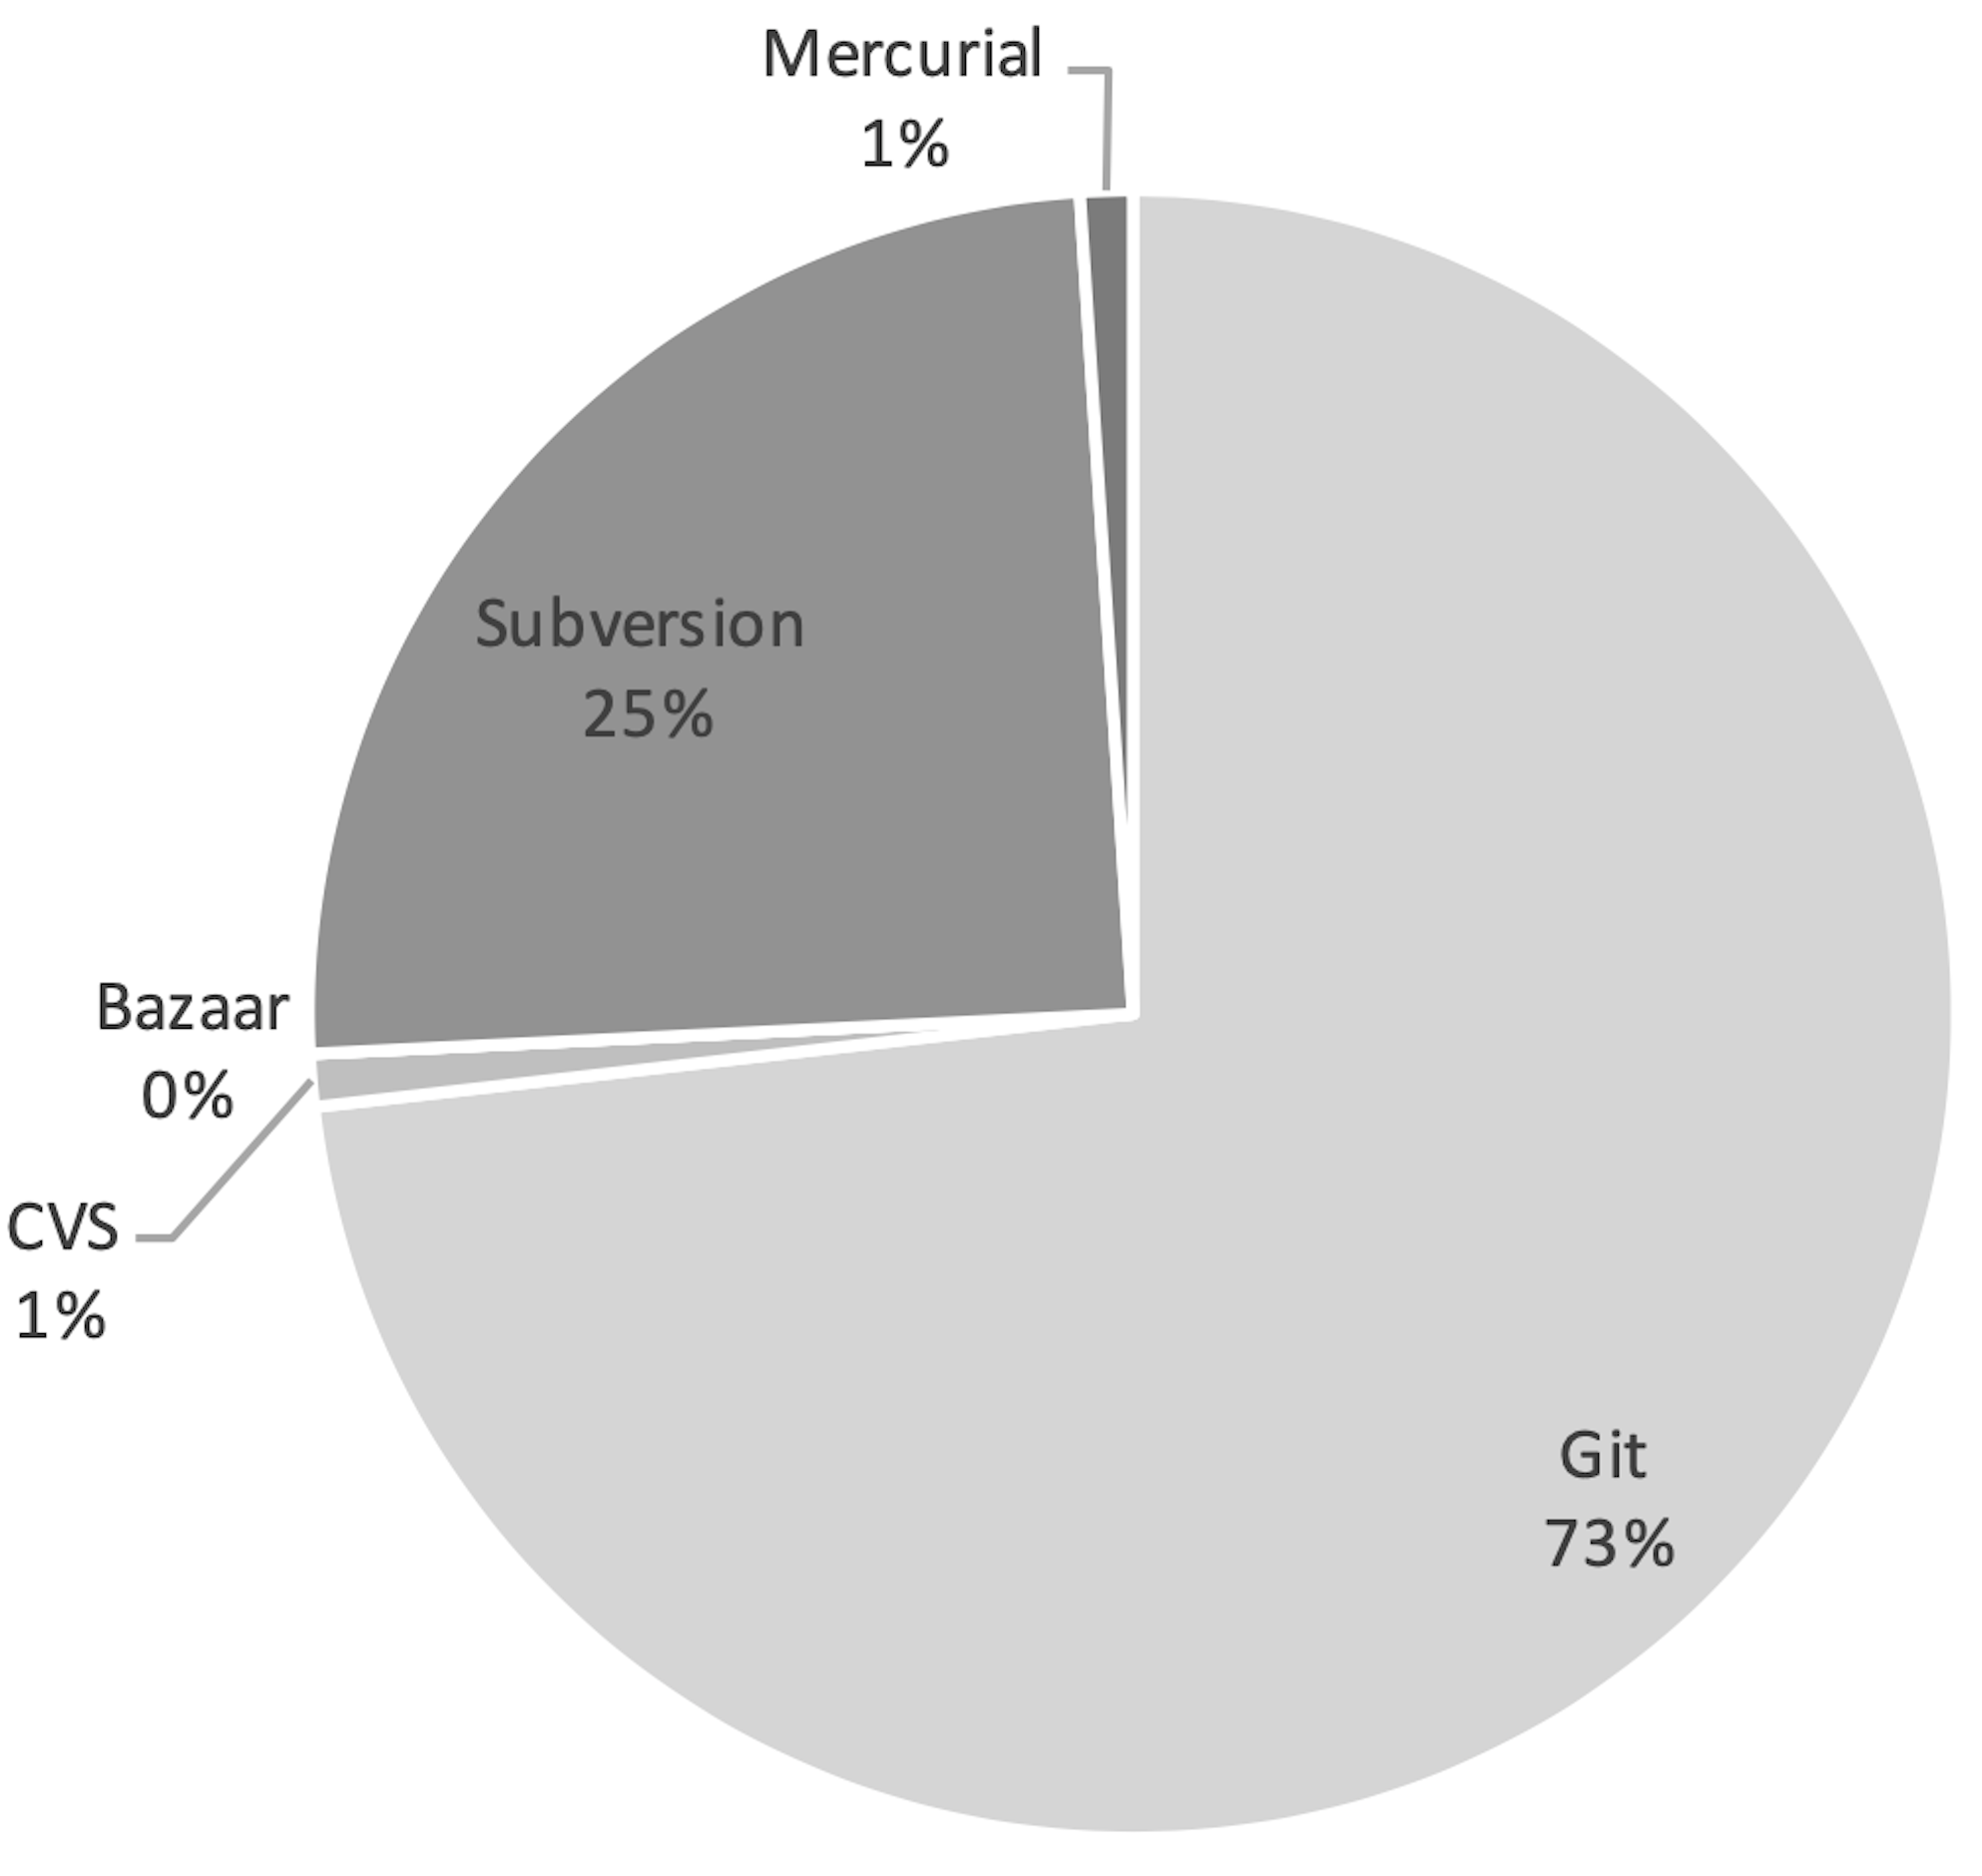
\includegraphics[width=1.1\marginparwidth]{ohloh.png}
    \caption{\label{fig:ohloh}Versionsverwaltungs-Tools im Ranking (nach Anzahl der Repositories) - Stand: 2020.}
\end{marginfigure}
\subsection{Versionsverwaltung}
Durch die Zusammenarbeit im Team an einem gemeinsamen Projekt werden Softwareentwickler häufig vor das Problem der Versionsverwaltung gestellt: Wie können mehrere Personen an einem gemeinsamen Projekt und z.T. sogar am selben Programm gleichzeitig arbeiten?
Wie können verschiedene Versionen eines Programms einheitlich und übersichtlich verwaltet werden? Und wie verfährt man möglichst effizient mit Code, welcher von unterschiedlichen Autoren geschrieben wurde und fügt diese zusammen? \newline Zur Lösung dieser Problemstellungen 
ist die Versionsverwaltung heutzutage in Softwareentwicklungsunternehmen kaum wegzudenken. Diese \enquote{ist ein System, welches die Änderungen an einer oder einer Reihe von Dateien über die Zeit hinweg, protokolliert, sodass man später auf eine bestimmte Version 
zurückgreifen kann} \cite{Scott-Chacon:2020aa}. \newline \newline Laut der Webseite Open Hub, welche zur Katalogisierung von Open-Source-Software verwendet wird und wie hier, den Anteil von Tools zur Versionsverwaltungs anhand der registrierten Daten indexiert, stellen Git (71\%) 
und Subversion (24\%) die populärsten, welche heutzutage eingesetzt werden, dar (s. Abbildung \ref{fig:ohloh}) \cite{Inc.:2020aa}, weswegen diese in den folgenden Unterkapiteln kurz angesprochen werden.
\pagebreak
\subsubsection{Git} \label{git}
Git\sidenote{\url{https://git-scm.com}} ist eine freie Software zur Versionsverwaltung \cite{Git:2020aa}. Die grundlegende Funktion unterscheidet hierbei zwischen der lokalen, zentralen und verteilten Versionsverwaltung: Die lokale Versionsverwaltung befasst sich dabei mit der \enquote{[Verwaltung] aller Änderungen relevanter Dateien in einer Datenbank} \cite{Scott-Chacon:2020aa}, wohingegen die
zentrale mit dem Problem der Kooperation mit anderen Entwicklern an gemeinsamer Software beschäftigt ist \cite{Scott-Chacon:2020aa}. Der letzte Punkt der verteilten Verwaltung behandelt das vollständige Kopieren eines sogenannten \enquote{Repositories} (dt. \textit{Quelle bzw. Lager von Software})
von einem Server anstatt lediglich den letzten Stand zu beziehen \cite{Scott-Chacon:2020aa}. Unter Git wird das Hauptverzeichnis als \enquote{master} bezeichnet, wohingegen die Versionierungen hiervon als \enquote{Branches} (vgl. Abbildung \ref{fig:git}), betitelt werden.

\subsubsection{Subversion} \label{svn}
Apache Subversion\sidenote{\url{https://subversion.apache.org}} (kurz: SVN) ist ebenfalls eine freie Software zur Versionsverwaltung von Dateien sowie Verzeichnissen, wodurch alte Versionen von Daten und eine Historie der verschiedenen Änderungen und Versionen an diesen betrachtet werden können \cite{Collins-Sussman:2004aa}.
Unter Subversion wird das Verzeichnis der \enquote{Hauptlinie} als \enquote{Trunk} definiert und seine Subverzeichnisse, wie auch schon unter Git, als \enquote{Branches}.
\begin{marginfigure}
    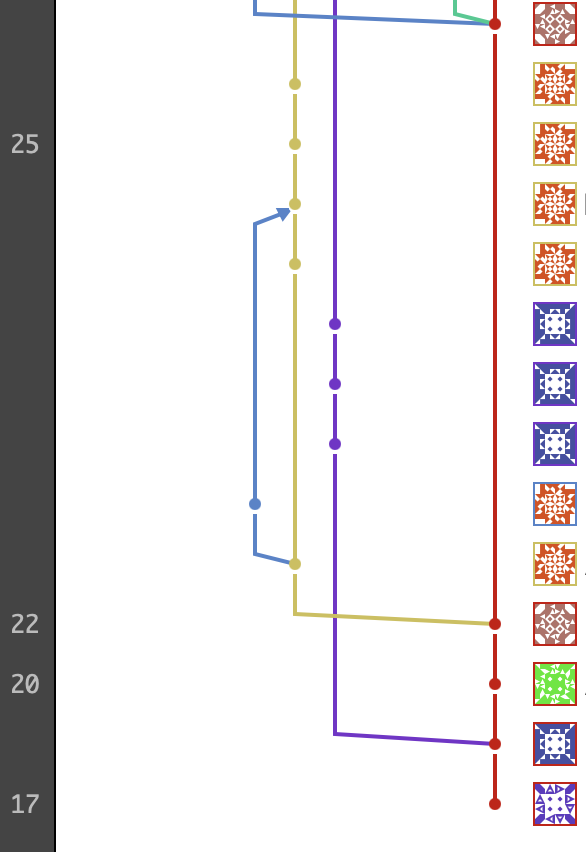
\includegraphics[width=1.1\marginparwidth]{git.png}
    \caption{\label{fig:git}Beispielhafte Historie einer Versionsverwaltung (hier: Git; Verschiedene Profilbilder repräsentieren einzelne Commit-Autoren, Abzweigungen repräsentieren Branches))}
\end{marginfigure}

